\documentclass[12pt,fleqn]{article}\usepackage{../../common}
\begin{document}
Ders 2.08

[Lineer problemler atlandı]

Şimdi gayrı lineer problemlere gelelim. Alttaki model denkleme bakalım,

$$
u_t + u u_x = 0
\mlabel{1}
$$

Bu denklem ile daha önce gördüğümüz alttaki denklem arasındaki fark bariz,

$$
u_t = c u_x
$$

Üstteki yatay iletim (advection) denkleminde sabit bir hız var, $c$. Ama iki
üstteki durumda hız $-u$, ya da $c$'nin yerine $-u$ koymuş oluyoruz.  O gayrı
lineer denklemi analiz etmek istiyoruz, daha önce olduğu gibi analitik olarak
çözmek isteriz, eğer mümkünse bir formüle erişmek isteriz.. Karakteristik
çizgiler bağlamında neler olduğuna bakmak isteriz.. Sonuçta tek bir uzay
değişkeni ve tek bir denklem var, buradan karakteristiklere bakarak işin
özünü görmek mümkün olmalı.

Ana denkleme eşdeğer olan bir form görelim,

$$
\frac{\partial u}{\partial t} +
\frac{\partial }{\partial x}
\underbrace{ \left( \frac{u^2}{2} \right)}_{f(u)} = 0
$$

Hatta üstteki forma daha ``doğru'' form ismi verilebilir, eğer onu açsak (1)'e
erişirdik fakat üstteki denklemdeki parantez içindeki kısmın fiziksel bir anlamı
var, o kısma akış (flux) ismi veriliyor.

Fakat göreceğiz ki bu diferansiyel denklem aynı noktada iki tane çözüm ortaya
çıkartabiliyor, ve onlardan birini seçmemiz gerekiyor. Diğer bir deyişle çözüm
süreksiz (discontinuous) hale gelebiliyor. Mükemmel pürüzsüz bir başlangıç
fonksiyonu bir süre sonra süreksiz oluyor. Sürekli başlıyoruz, çözüm
karakteristik çizgiler üzerinde sabit, fakat iki karakteristik çizgi birbiriyle
çakıştığında ne olur? Daha önce çakışma olmadı çünkü ana denklem o türde
değildi. Burada mümkün!

O durumu alta çizdim,

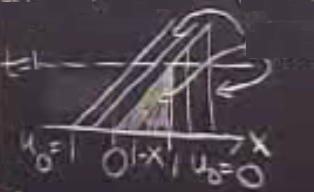
\includegraphics[width=15em]{compscieng_2_08_01.png}
























[devam edecek]
  
\end{document}
